\section{Realizzazione DBMS}

Un \textbf{\textcolor{purple}{DBMS}} è un sistema software che
gestisce grandi quantità di dati, si và incontro
a problemi di efficienza, che sono \emph{\textcolor{purple}{persistenti}}, quindi il sistema
deve garantire affidabilità, e \emph{\textcolor{purple}{condivisi}}, in questo caso deve gestire il
controllo degli accessi e della concorrenza. La condivisione dei dati
è importante perchè permette di evitare la ridondanza dei dati (che porterebbe ad un spreco di memoria),
ma può anche portare a problemi di inconsistenza, dato che se si hanno tante copie
di un dato, una modifica di una sola delle copie deve essere propagata nelle altre.

A causa della sua dimensione, un database risiede normalmente
sui dischi, e prima che i suoi dati debbano essere elaborati dal
DBMS, questi devono essere trasferiti in memoria centrale. Questo
trasferimento non coinvolge le singolo tuple ma è effettuato
a \textcolor{purple}{blocchi} o \textcolor{purple}{pagine}.

Un \textcolor{purple}{blocco}, fisicamente, è una sequenza
continua di settori di una traccia, costituendo l'unità di trasferimento
dati da e per la memoria principale. La dimensione tipica è tra i 4 - 64 KB.

\paragraph{\textcolor{purple}{Struttura della Pagina}} Una pagina, logicamente,
è formata da alcune informazioni di servizio e da un'area dove sono contenuti
dei \emph{record}. Il riferimento ad un record, chiamato \textbf{RID} è formato
dalla coppia (\textbf{PID} della pagina, posizione del record nella pagina).

\begin{figure}[H]
    \centering
    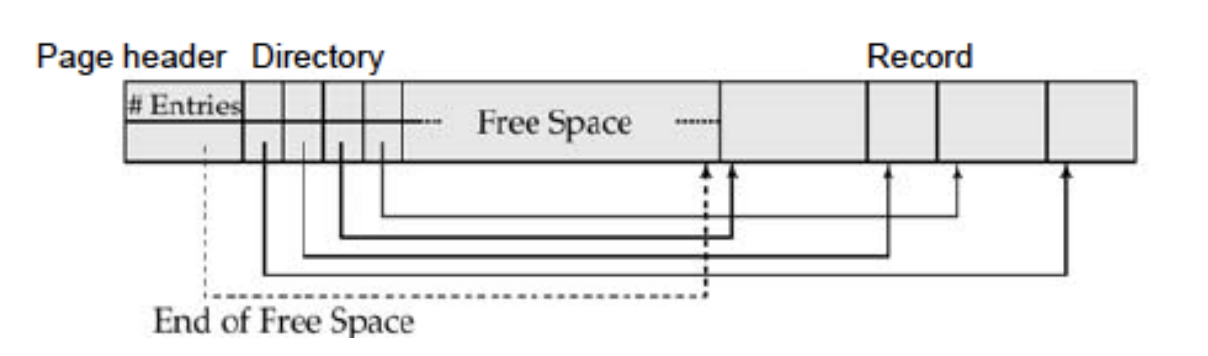
\includegraphics[scale=0.55]{img/rid.png}
\end{figure}

La \textcolor{purple}{directory} contiene un puntatore per ogni record
della pagina, in questo modo è possibile riallocare il record nella pagina
senza modificare il \textbf{RID}.

\subsection{Gestore Memoria}

L'architettura a livello fisico è la seguente.
\begin{figure}[H]
    \centering
    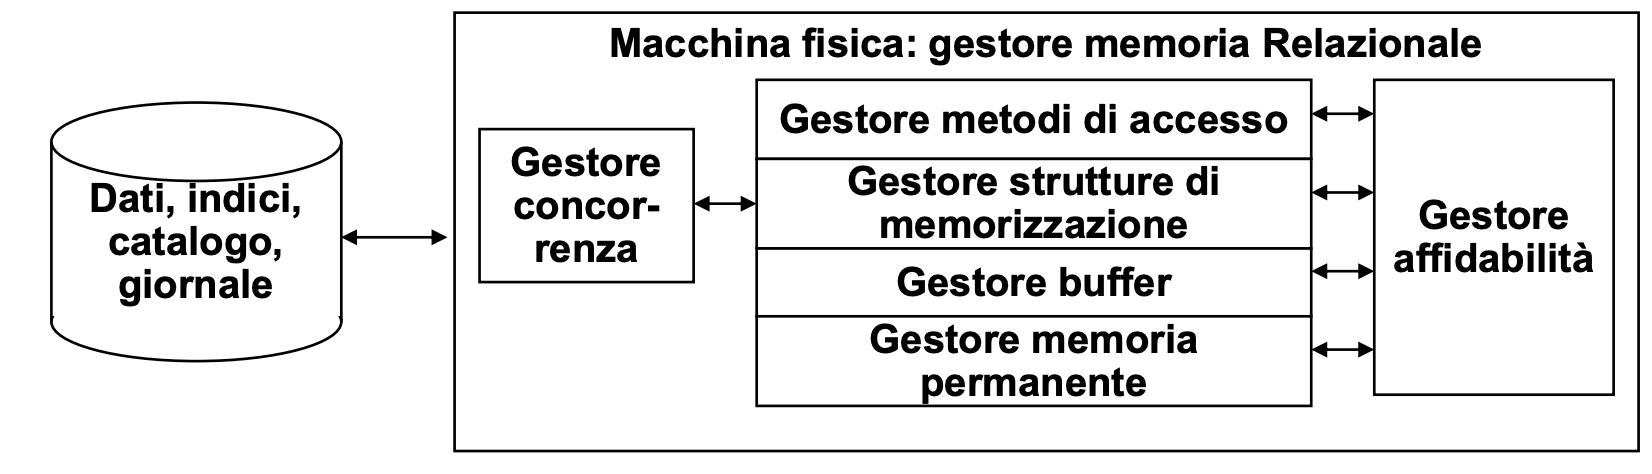
\includegraphics[scale=0.4]{img/macchina_fisica.png}
\end{figure}

\begin{itemize}
    \item \textcolor{purple}{Gestore Memoria Permanente}: fornisce un'astrazione della memoria
        permanente sotto forma di insiemi di file logici di blocchi fisici, nascondendo
        le caratteristiche dei dischi e dell'OS.
    \item \textcolor{purple}{Gestore del Buffer}: si occupa del trasferimento delle pagine
        tra la memoria temporanea e quella permanente, offrendo ai livelli superiore
        una visione della memoria permanente come un insieme di pagine utilizzabili in quella temporanea.
        In questo modo viene nascosta l'operazione di trasferimento.
            \begin{figure}[H]
                \centering
                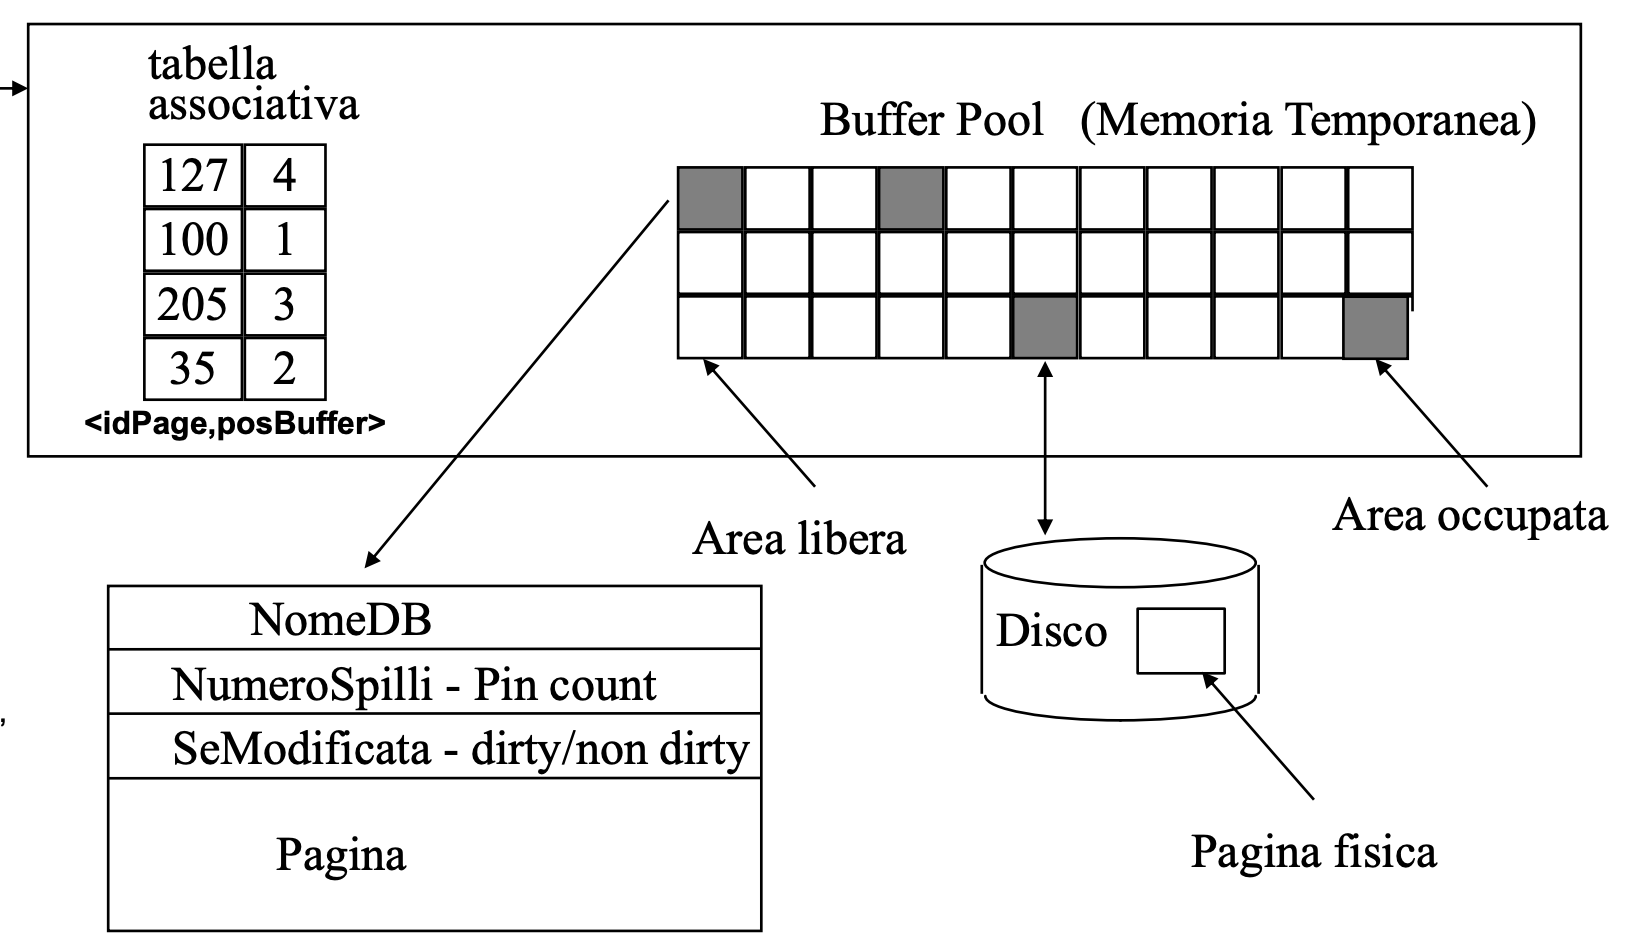
\includegraphics[scale=0.4]{img/buffer.png}
            \end{figure}
        Nell'header della pagina presente nella memoria temporanea, \emph{Pin Count}
        viene incrementato se la pagina viene richiesta e decrementato se viene rilasciata.
        Vengono utilizzate alcune primitive:
        \begin{itemize}
            \item \verb|getAndPinPage(x)|: indica la richiesta al buffer della pagina
                con \verb|idPage = x| e viene incrementato il \verb|pin count| relativo a quella
                pagina per indicarne l'uso.
            \item \verb|unPinPage(x)|: rilascia una pagina e decrementa il \emph{pin count}.
            \item \verb|setDirty(x)|: imposta il bit \verb|dirty| a 1, che indica se la pagina
                è stata modificata.
            \item \verb|flushPage(x)|: forza la scrittura della pagina su disco ed imposta il bit \verb|dirty|
                a 0.
        \end{itemize}
    \item \textcolor{purple}{Gestore Strutture di Memorizzazione}: ogni tipo di organizzazione ha i suoi
        pro e contro, basandoci sul costo delle operazioni che effettuiamo sui dati e sulla sua occupazione
        in memoria.
        \begin{itemize}
            \item \textcolor{purple}{Organizzazione Seriale} o \textcolor{purple}{Heap File}: i dati sono memorizzati
                in modo casuale uno dopo l'altro, il costo in memoria è basso ma è poco efficiente per le operazioni.
            \item \textcolor{purple}{Organizzazione Sequenziale}: i dati vengono ordinati sul valore di uno o più attributi,
                le inserizioni fanno perdere l'ordinamento, ma le ricerche sono più veloci, dato che si applica la ricerca
                binaria. Se un file contiene un numero di pagine uguale a \verb|b| allora occorreranno un numero di accessi
                uguale a $\log_{2}{b}$ per individuare il record.
            \item \textcolor{purple}{Organizzazioni Per Chiave}: in queste organizzazioni, noto il valore di una
                chiave si trova il record di una tabella con un numero di accessi al disco che dovrebbe essere
                idealmente uguale ad 1.
        \end{itemize}
\end{itemize}

\subsection{Organizzazioni Per Chiave}

\subsubsection{Hash File}
In un file hash, i record vengono allocati in una pagina il cui indirizzo dipende dal
valore di chiave del record stesso. Ad esempio, se un record ha chiave $k$ allora si inserisce
nella pagina di indirizzo $H(k)$, dove $H(k) = k \mod NrPage$.

Le collisioni sono gestite con delle \emph{Linked List}. Questa organizzazione è la più
efficiente se si considera solo l'accesso diretto basato sui valori della chiave con condizioni
di uguaglianza. Non è efficiente invece per ricerche basate su intervalli o su attributi diversi dalla
chiave. Inoltre è un'organizzazione \textcolor{purple}{procedurale statica}, quindi funziona solo
su file la cui dimensione varia poco nel tempo.

Invece, gli svantaggi che riguardano puramente la struttura dipendono dal numero di pagine, se è troppo
piccolo rispetto alla dimensione del database si hanno frequenti collisioni, altrimenti se è troppo grande il
fattore di riempimento delle pagine è molto basso.

\subsubsection{Metodo Tabellare}

Si usa un \textcolor{purple}{indice}, ovvero un insieme ordinato
di coppie \verb|(k, r(k))|, dove \verb|k| è un valore della chiave ed \verb|r(k)|
è un riferimento al record con chiave \verb|k|. Gli indici possono essere
su più attributi. L'indice viene gestito con una struttura chiamata
$B^+-tree$. Prima di vedere i $B^+-tree$, vediamo i $B-tree$, dove fissato l'ordine
$p$, questi rappresentano degli alberi di ricerca dove ogni nodo interno ha questa forma:
\begin{equation*}
    <P_1, <K_1, Pr_1>, P_2, <K_2, Pr_2>, \dots, <K_{q-1}, Pr_{q-1}>, P_q>
\end{equation*}
dove $q \leq p$. I $P_i$ sono chiamati \emph{tree pointer} ovvero rappresentano
un puntatore ad un altro node del $B-tree$, $K_i$ è la chiave di ricerca, e $Pr_i$
è un \emph{data pointer}, ovvero è un puntatore ad un record il cui campo \emph{chiave di ricerca}
è uguale a $K_i$ oppure ad una pagine che contiene tale record.
Per ogni nodo vale la proprietà $K_1 < K_2 < \dots < K_{q-1}$, e deve avere al massimo
$p$ \emph{tree pointer}.

\begin{figure}[H]
    \centering
    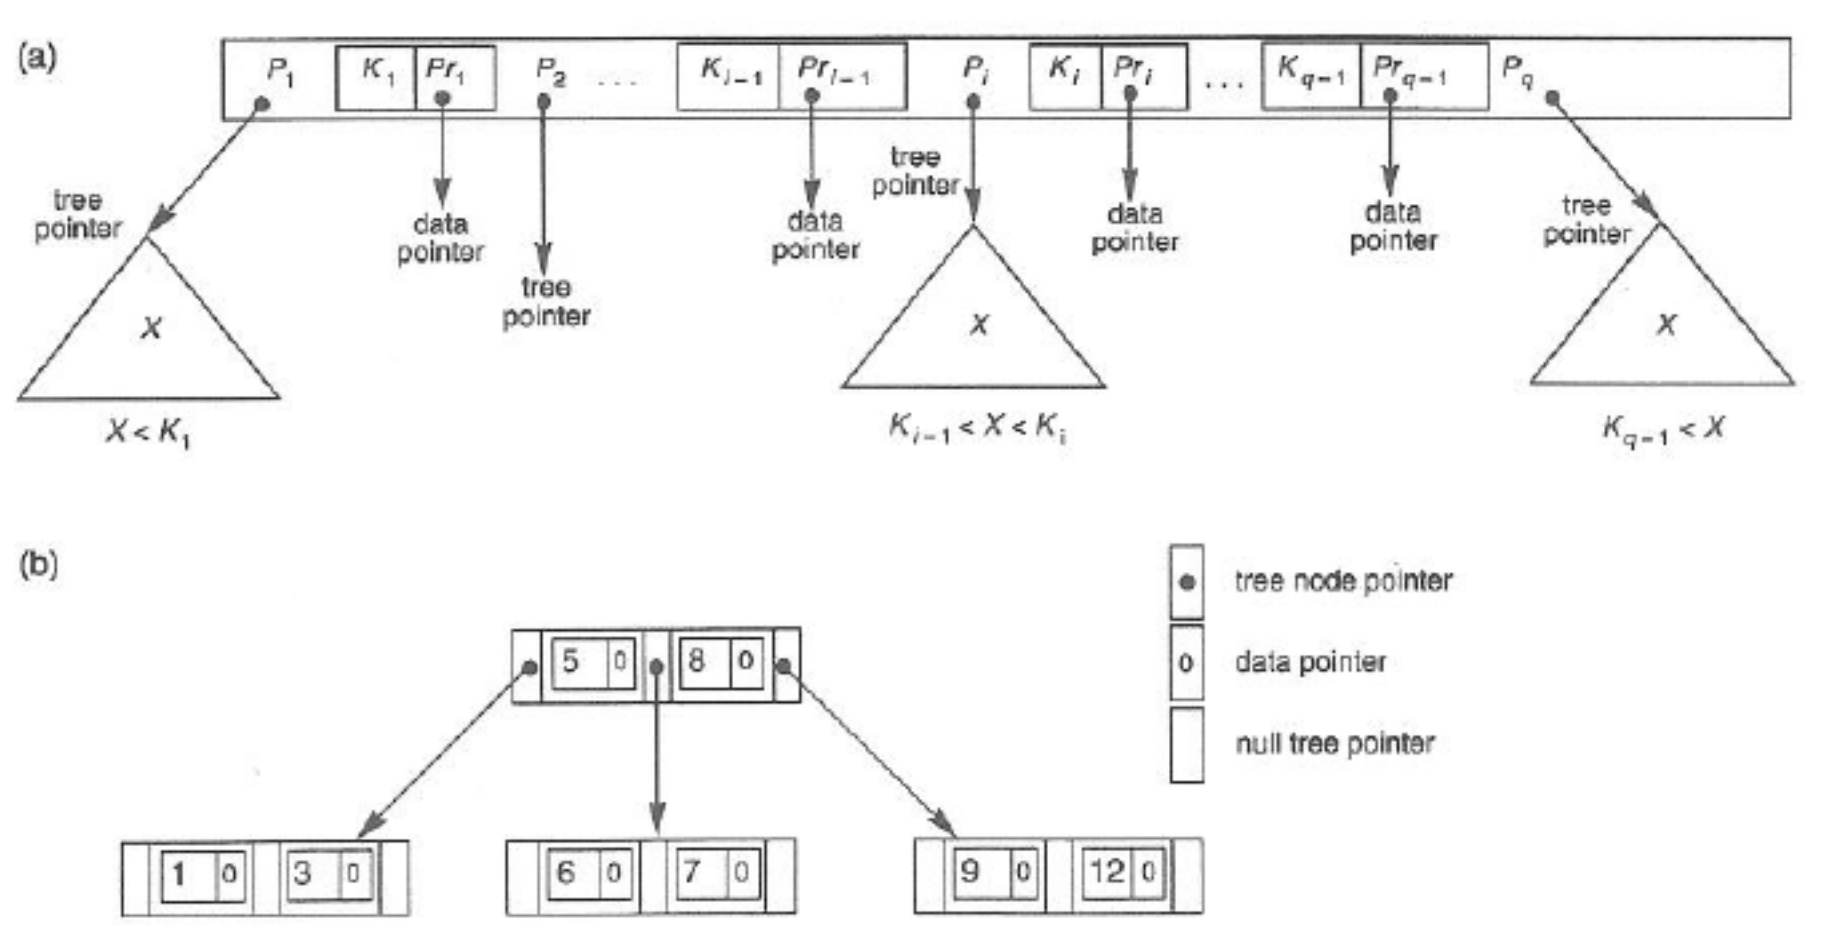
\includegraphics[scale=0.37]{img/btree.png}
\end{figure}

Per tutti i valori $X$ della chiave di ricerca che appartengono al
sottoalbero puntato da $P_i$ vale che:
\begin{equation*}
    K_{i-1} < X < K_i \;\;per\; 1 < i < q
\end{equation*}
\begin{equation*}
    X < K_i \;\;per\; i = 1
\end{equation*}
\begin{equation*}
    K_{i-1} < X \;\;per\; i = q
\end{equation*}

I vincoli che il $B-tree$ deve rispettare, che lo differenziano da un normale
albero di ricerca sono:
\begin{itemize}
    \item La radice ha almeno due \emph{tree pointer} a meno che non sia l'unico nodo.
    \item Ogni nodo, esclusa la radice, ha almeno $\lceil \frac{p}{2} \rceil$
        \emph{tree pointer}.
    \item Tutti i nodi foglia sono posti sullo stesso livello.
\end{itemize}
Questi vincoli garantiscono che il $B-tree$ sia bilanciato. \\

I $B^+-tree$, sono essenzialmente dei $B-tree$ dove i \emph{data pointer} sono memorizzati
esclusivamente nei nodi foglia dell'albero. Quindi, fissato l'ordine $p$, ogni nodo interno
ha la seguente forma:
\begin{equation*}
    <P_1, K_1, P_2, K_2, \dots, P_{q-1}, K_{q-1}, P_q>
\end{equation*}
con $q \leq p$.
Un'altra piccola differenza è che per ogni valore $X$ della chiave di ricerca
puntata da $P_i$ si ha che:
\begin{equation*}
    X \leq K_i \;\;per\; i = 1
\end{equation*}
\begin{equation*}
    K_{i-1} < X \leq K_i \;\;per\; 1 < i < q
\end{equation*}
\begin{equation*}
    K_{i-1} < X \;\;per\; i = q
\end{equation*}

\begin{figure}[H]
    \centering
    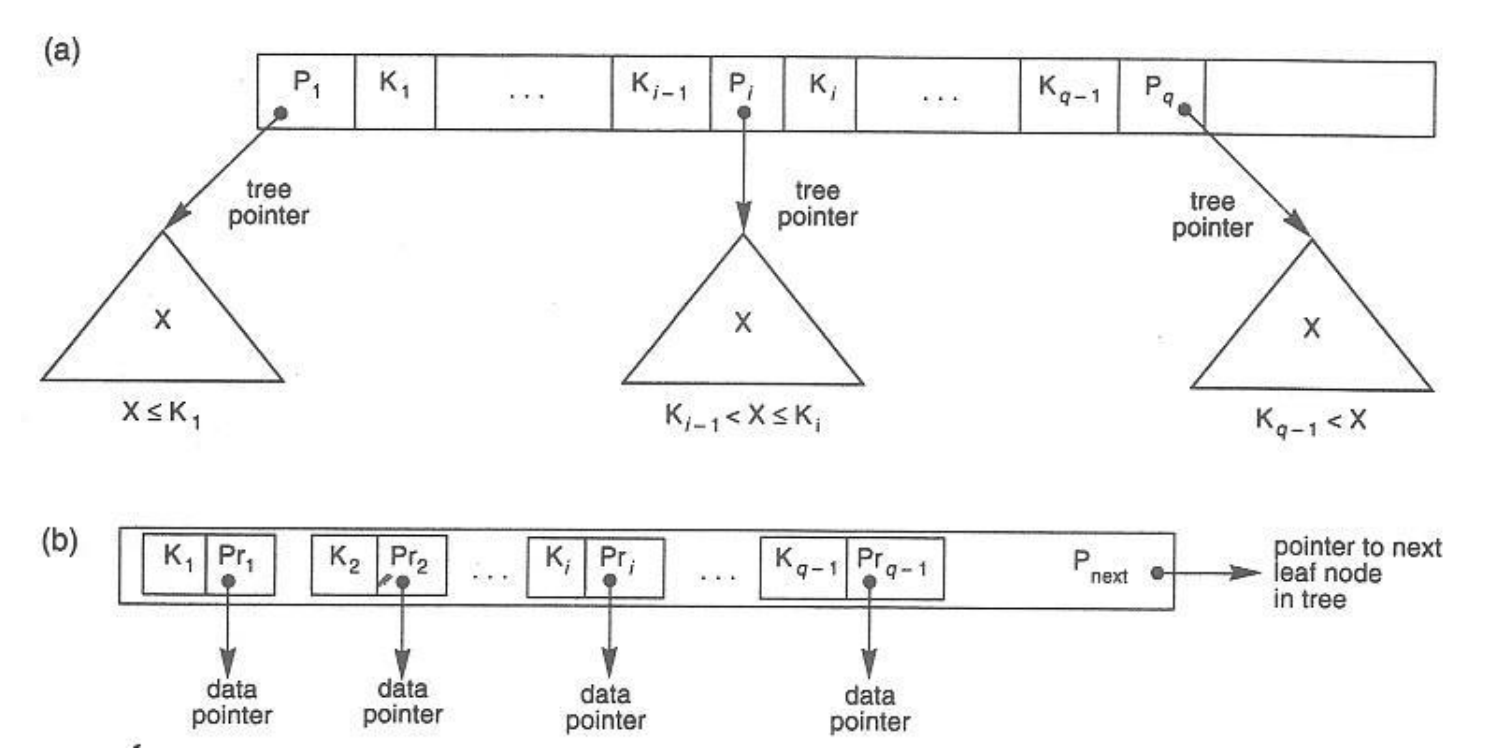
\includegraphics[scale=0.46]{img/b+tree.png}
\end{figure}

La struttura dei nodi foglia è la seguente:
\begin{equation*}
    <<K_1, Pr_1>, <K_2, Pr_2>, \dots, <K_q, Pr_q> P_{next}>
\end{equation*}
dove $q \leq p_{leaf}$ e dove vale sempre $K_1 < K_2 < \dots < K_q$.
$P_{next}$ è un \emph{tree pointer} che punta al successivo nodo foglia
del $B^+-tree$. Ogni $Pr_i$, invece, è un \emph{data pointer} che punta al record
con campo di ricerca uguale a $K_i$, a un blocco contenente tale record, o a un blocco
di puntatori ai record con campo di ricerca uguale a $K_i$, se il campo di ricerca non è una
chiave. Ogni nodo foglia ha almeno $\lceil \frac{p_{leaf}}{2} \rceil$ valori. 

Ovviamente è importante sottolineare che gli alberi stessi sono memorizzati su disco,
assegnando ad ogni nodo una pagina. \\

Esistono due tipologie di indici ad albero:
\begin{itemize}
    \item \textcolor{purple}{Indici Statici}: la struttura ad albero viene creata sulla
        base dei dati presenti nel database e non viene più modificata se non periodicamente.
    \item \textcolor{purple}{Indici Dinamici}: la struttura ad albero viene aggiornata ad
        ogni operazione di inserimento e cancellazione.
\end{itemize}

Gli indici si possono anche distinguere in:
\begin{itemize}
    \item \textcolor{purple}{Indici Primari}: in questo caso la chiave di ordinamento del
        file sequenziale coincide con la chiave di ricerca dell'indice. È costituito da un insieme
        di coppie \verb|<K(i), RID(i)>|, dove il primo campo è la chiave primaria ed è dello stesso tipo
        del campo chiave di ordinamento, mentre il secondo campo è un puntatore ad un blocco del disco.
    \item \textcolor{purple}{Indici Secondari}: qui invece la chiave di ordinamento e quella
        di ricerca sono diverse. Questo indice può essere definito su un
        campo che non è chiave ma è chiave candidata, quindi ha valori univoci, oppure su un campo
        che ha valori duplicati. In questo caso il primo campo della coppia è chiamato campo di indicizzazione.
\end{itemize}